%!TEX root = ../dissertation.tex
\chapter{Experiment 1: Effect of Retinal Orientation on Fixational Stability and Accuracy}

\section{Brief Introduction}

There is a substantial literature regarding the effects of orientation relative to the fovea on functional visual performance. Acuity, contrast sensitivity \citep{skrandies_1987}, attentional resolution \citep{rezec_2004}, the volitional control of ``sustained'' attention  \citep{mackeben_1999,altpeter_2000}, chromatic sensitivity \citep{levine_2005}, motion sensitivity \citep{levine_2005,edwards_1993}, and crowding \citep{he_1996} all appear to vary as a function of orientation relative to the fovea. However, there is much less available concerning similar effects on oculomotor control either for PRL or PPRL. This experiment has therefore been designed to address three primary research questions:

\begin{enumerate}
\item Can we induce a pPRL?
\item Will explicit training at the pPRL site improve fixational stability and reduce the magnitude of oculomotor errors with respect to targets over time?
\item Will any effect of explicit pPRL training transfer to a new pPRL following a 90\degree orientation shift?
\end{enumerate}

The first question is of interest as a confirmation of the existing literature in this area. If it is possible to induce a pPRL experimentally, then the second question follows naturally: will explicit practice with/use of this pPRL site enhance fixational stability? Finally, the third question is of interest as a form of biological validation: the progression of retinal disease often forces sufferers to develop new PRL locations as old sites are claimed by the growth of lesions. By forcing subjects to form pPRL at a new location during their second training set, we examine the extent to which pPRL use represents a kind of underlying learned skill that can survive the destruction of individual pPRL sites.

\section{Methods}
Eye movement data for this project were collected using an SR Research Eyelink 1000 infrared eye tracking system. Stimuli were presented on a 68.58cm diagonal width ASUS VG278He monitor running at a 144Hz refresh rate. Subjects were seated at a distance of 55cm from the display, which therefore subtended a 54\degree horizontal visual angle. Subjects' heads were stabilized during the experiment using an Eyelink-supplied chin and forehead rest. Stimuli were generated, displayed, and modified in real time on the basis of input from the Eyelink through the use of the MATLAB Psychtoolbox \citep{brainard_1997} and Eyelink Toolbox \citep{cornelissen_2002}. Data were sampled at a rate set to match the refresh rate of the monitor. Subjects' gaze profile was calibrated to the display using the standard nine-point calibration protocol provided with the Eyelink before each experimental session began. 

Eight participants (six women, two men) with normal or corrected-to-normal vision were recruited from the authors' laboratory and from the undergraduate population at Northeastern University. Undergraduates received course credit towards the completion of their introductory psychology course in exchange for their participation. All were naive to the purposes of the study at intake and indicated their willingness to participate by signing an informed consent document associated with a protocol approved by the University Ethics Board. The Northeastern University Ethics Board evaluated the protocol and confirmed that this research adhered to the tenets of the Declaration of Helsinki.

Participants completed a total of 400 training trials, split into two training sessions of 200 trials each. Sessions were separated by a period of roughly one week (mean 8.6 days, sd 3.2 days). Within a session, each subject completed four blocks of 50 trials. Between blocks, they were asked to rest for as long as they felt they needed. All were then re-calibrated using the same nine-point calibration procedure before continuing the experiment. Trials lasted for fifteen seconds. During a trial, subjects were asked to center a gaze contingent ring over a motionless fixation target and to maintain that position for as long as they were able (see Figure 1 for a schematic representation of the task). The fixation target was a full-contrast red (RGB: [255,0,0]) circle with a diameter of 24 pixels. The line forming the gaze contingent ring was three pixels wide and drawn as a full contrast green (RGB: [0,255,0]). Trials fell into one of two orientation conditions: ``east'' or ``south''. In the east, the ring was drawn 6.4\degree (128 pixels) to the right, and in the south 6.4\degree below, the foveated point of regard. Each session contained trials associated with one condition. At the beginning of the second training session, subjects switched conditions. The order in which they were completed was counterbalanced between subjects.

Within a trial, if subjects remained ``on target'' over the fixation target for a period of 100ms, the diameter of the ring was reduced by a factor of 1.18, making the task more difficult. Similarly, if they fell ``off target''during the same period, its diameter was increased to an equivalent degree, making the task easier. Finally, they were prevented from using their fovea to assist them by removing the fixation target from the screen if their foveated point of regard fell within a 2\degree radius of the target center. This approximated an absolute central scotoma of the same size. Performance on the task was measured in two ways. First, gaze ``accuracy'' was assessed in terms of the within-trial median log-transformed (natural log or base \textit{e}) euclidean distance between the center of the ring and the center of the target. Second, their gaze ``stability'' with respect to the target was assessed in terms of the area within a fitted isocontour containing 95\% of the gaze points within a trial (See \cite{castet_2012} for a full description of this method). Figure ~\ref{chap_1_outcome_figure} is a schematic representation of the two performance measures and their relationship to each other.

\begin{figure}[!htbp]
\centering
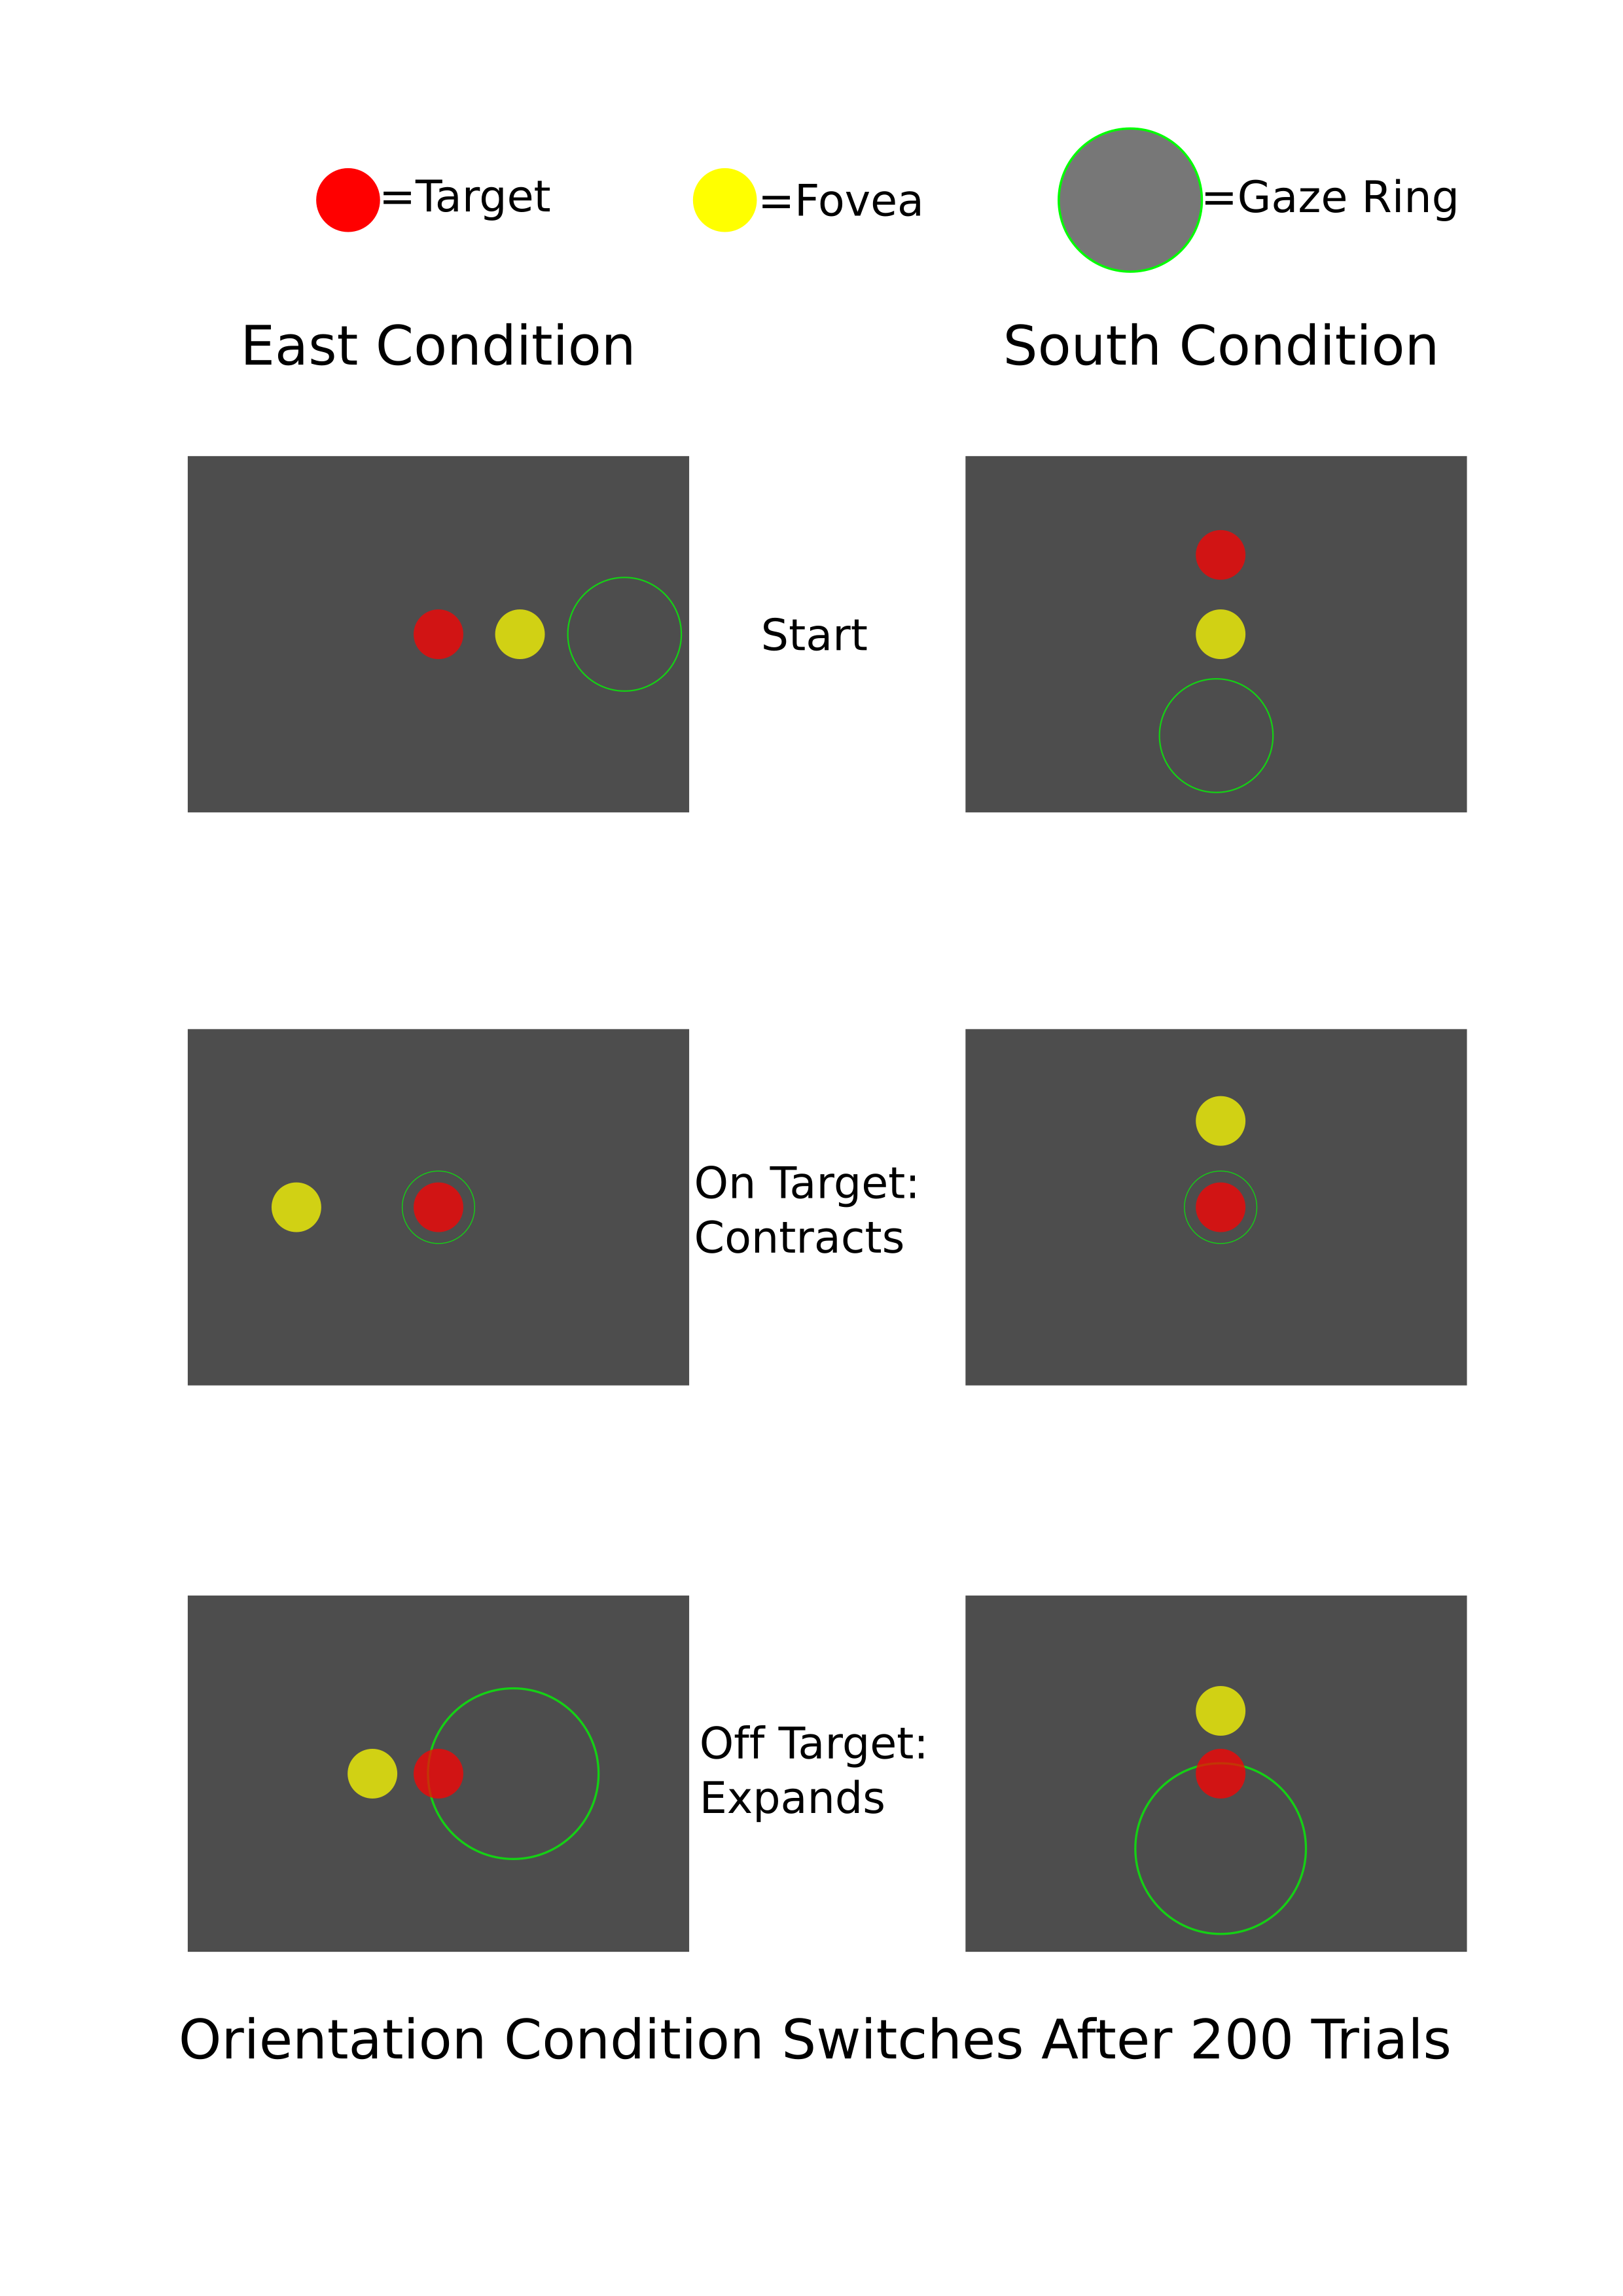
\includegraphics[width=.75\linewidth,height=.75\textheight,keepaspectratio]{figures/chapter_1/demo_image.png}
\caption[Schematic Depiction of Experimental Design for Experiment 1]{Subjects completed a training session composed of 200 trials in one orientation condition, then completed a second session in the other approximately a week later. Keeping the ring on target caused it to contract after 100ms, making the task harder. Falling off target during the same period caused it to expand, making the task easier. Recorded foveal position (yellow circle) was not shown to research participants.}\label{chap_1_demo_figure}
\end{figure}
 
\begin{figure}[!htbp]
\centering
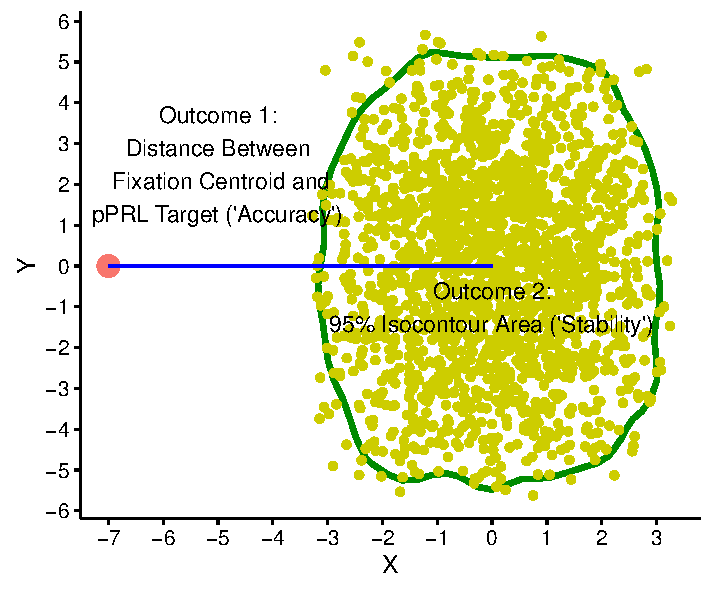
\includegraphics[width=.75\linewidth,height=.75\textheight,keepaspectratio]{figures/chapter_1/outcomes_figure.pdf}
\caption[Schematic Depiction of Outcome Measures and Their Relationship for All Experiments.]{The distance between the center of the red target dot and the centroid of the cluster of gaze points (blue line) is the subject's gaze ``accuracy'' with respect to the target. The region highlighted in green is a fitted isocontour that contains 95\% of the available gaze points(yellow circles), representing a subject's gaze ``stability'' to the target. Data are simulated and presented in normalized, arbitrary units.}\label{chap_1_outcome_figure}
\end{figure}

Data from this experiment were analyzed using the \textit{R} statistical programming language. First, hierarchical linear models (HLMs) were fitted to both the stability and error data. The structure of both models included fixed effects terms for the total block number (one to eight), orientation condition, and an interaction term between orientation condition and whether it was the first or second training session. Both also included by-subject random effects and slopes to capture potential individual differences in both baseline performance and rate of learning. This approach also allowed us to control significant multi-collinearities in the data at a number of scales resulting from the repeated-measures design of the experiment and correlations between sample-to-sample deviations from the target. Second, to assess the degree to which effects of training survived the inter-set period and transferred to the new training location, we used paired t-tests comparing subjects' performance in both outcome measures between the first block of the first training session (block 1) and the first block of the second (block 5). 

\section{Results}

One subject (GM) was excluded from all analyses of stability data as raw gaze position data was not collected for them. Average by-block, across-subject performance for both outcome measures is presented in Figures 3a and 3b. In both figures, points are mean performance across subjects and trials within a block of training; error bars are fitted 95\% confidence intervals. In both cases, a similar pattern of performance emerged across time: rapid improvement between the first and second blocks of training, then a leveling off toward the end of the first training session. At the beginning of the second session, both stability and accuracy performance fell sharply, then ultimately improved to levels beyond that achieved during the first session of training.

\begin{figure}[htbp]
\centering
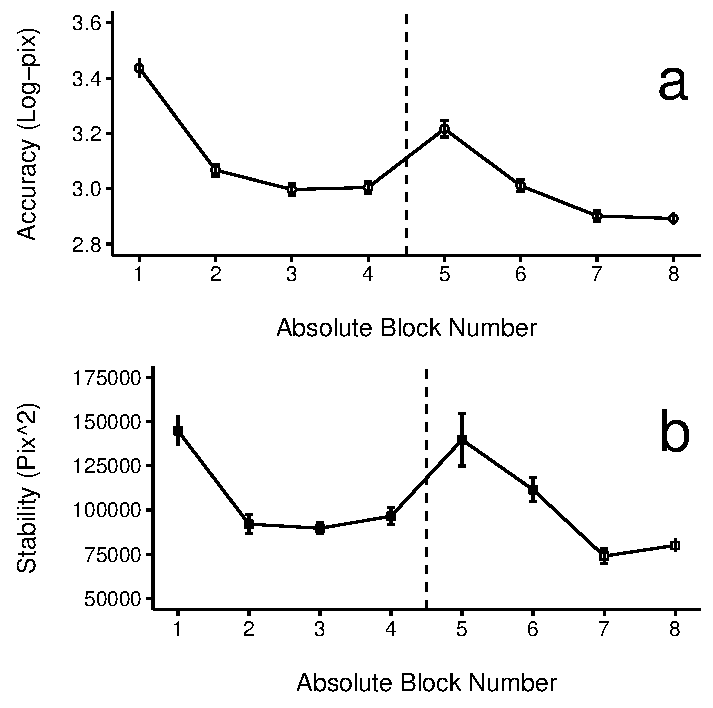
\includegraphics[width=.75\linewidth,height=.75\textheight,keepaspectratio]{figures/chapter_1/outcome_by_block.pdf}
\caption[Experiment 1: Outcomes by Block]{\textbf{a}: mean log-transformed median distance (pixels) between the centers of the target and ring as a function of training block number across subjects and trials. Dots represent within block means, and bars 95\% confidence intervals. The dashed line between blocks 4 and 5 on the x-axis is the point at which subjects switched orientation conditions. \textbf{b}: mean stability performance (pixels-squared) within blocks and across subjects. The elements of this figure are otherwise the same as in \textbf{a}.}\label{chap_1_outcome_by_block}
\end{figure}

In the fitted model for the error data, only the absolute block number term attained statistical significance (coefficient value: -.122, \textit{p}\textrm{\textless0.01}). This suggests that the training was associated with significant improvements in fixational accuracy at the pPRL site. The parameter associated with training block number indicates that after completing all eight blocks, the magnitude of subjects' errors with respect to the target fell by a factor of nearly one natural log unit, i.e. an almost three-fold (2.7) improvement. For the stablility data, the absolute block number was also the only parameter in the fitted model that reached statistical significance (coefficient value: -18,192.570, \textit{p}\textrm{\textless0.01}), indicating that stability also significantly improved as a function of training. The full model fit for both outcome measures is presented in Table ~\ref{chap_1_outcome_table}.

\begin{table}[!htbp] \centering
\resizebox{.75\linewidth}{!}{\begin{minipage}{\linewidth}
  \caption{Experiment 1: Outcome Model Fits} 
  \label{chap_1_outcome_table} 
\begin{tabular}{@{\extracolsep{5pt}}lcc} 
\\[-1.8ex]\hline 
\hline \\[-1.8ex] 
 & \multicolumn{2}{c}{\textit{Dependent variable:}} \\ 
\cline{2-3} 
\\[-1.8ex] & Accuracy (Log Pixels) & Stability (Pixels Squared) \\ 
\\[-1.8ex] & (1) & (2)\\ 
\hline \\[-1.8ex] 
 Absolute Block Number & $-$0.122$^{***}$ & $-$18,192.570$^{***}$ \\ 
  & (0.019) & (4,925.740) \\ 
  Orientation Condition & $-$0.066 & $-$66,751.440 \\ 
  & (0.279) & (47,161.760) \\ 
  First or Second Session of Training & 0.292 & 17,493.600 \\ 
  & (0.275) & (45,566.800) \\ 
  Orientation x First or Second Session of Training & 0.151 & 96,261.980 \\ 
  & (0.545) & (88,352.310) \\ 
 \hline \\[-1.8ex] 
Observations & 3,199 & 2,800 \\ 
Log Likelihood & $-$1,999.204 & $-$36,839.610 \\ 
Akaike Inf. Crit. & 4,016.407 & 73,697.210 \\ 
Bayesian Inf. Crit. & 4,071.043 & 73,750.650 \\ 
\hline 
\hline \\[-1.8ex] 
\textit{Note:}  & \multicolumn{2}{r}{$^{*}$p$<$0.1; $^{**}$p$<$0.05; $^{***}$p$<$0.01} \\ 
\end{tabular}
\end{minipage} } 
\end{table} 

Figure ~\ref{chap_1_paired_t} presents means and 95\% confidence intervals across subjects and trials between blocks one and five. A two-tailed paired t-test comparing accuracy performance between these blocks produced a significant result (df=399,t=3.14,\textit{p}\=0.002); stability performance between them was not significantly different (df\textdblhyphen349,t\textdblhyphen0.4654,\textit{p}\textdblhyphen0.64). This suggests that stability performance gains may be less resistant to decay over time than accuracy performance, though recovery and improvement appears to resume quickly starting in the \textit{third} block of the second training session (block 7). 

\begin{figure}[htbp]
\centering
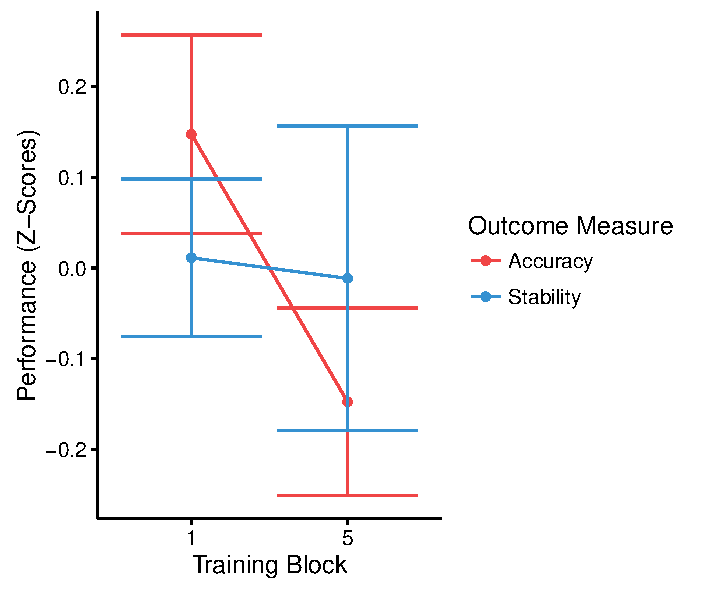
\includegraphics[width=.75\linewidth,height=.75\textheight,keepaspectratio]{figures/chapter_1/paired_t_results.pdf}
\caption[Experiment 1: Performance Comparison Between First Block of Both Sessions for Both Outcome Measures]{Means and 95\% confidence intervals for outcome measures 95\% fitted isocontour areas) between training block 1 (the first block of the first session) and training block 5 (the first block of the second training session). Data in this figure have been transformed to z-scores (mean zero, standard deviation of one) in order to set them on a shared scale.}\label{chap_1_paired_t}
\end{figure}

\section{Brief Discussion}

Our findings support the claim that is possible to train a pPRL in individuals with healthy retinas. We have also demonstrated that explicit oculomotor control training at this location can significantly improve subjects' fixational stability and accuracy with respect to a target. This effect of the training appears to persist over time and is robust to up to 90\degree changes in pPRL orientation relative to the fovea. We interpret the null findings with respect to the other model parameters for both outcome measures models to mean that neither orientation is intrinsically easier at baseline or that first training on one orientation facilitates transfer of learning to a second. 

These findings suggest a possible dissociation between oculomotor and functional vision maps. This has interesting implications for the development of our method as a training program to assist the visually impaired. If the center of the oculomotor control map -- and thus the site of the most precise eye movement control -- can effectively be shifted through training in any direction away from the fovea, then there may be no penalty in terms of functional vision associated with training a pPRL at a particular \textit{orientation} relative to another. In the second experiment in this series, we examined whether this claim would hold in terms of retinal \textit{eccentricity}.
